%%%%%%%%%%%%%%%%%%%%%%%%%%%%%%%%%%%%%%%%%%%%%%%%%%%%%%%%%%%%%%%%%%%%%%
% How to use writeLaTeX: 
%
% You edit the source code here on the left, and the preview on the
% right shows you the result within a few seconds.
%
% Bookmark this page and share the URL with your co-authors. They can
% edit at the same time!
%
% You can upload figures, bibliographies, custom classes and
% styles using the files menu.
%
%%%%%%%%%%%%%%%%%%%%%%%%%%%%%%%%%%%%%%%%%%%%%%%%%%%%%%%%%%%%%%%%%%%%%%

\documentclass[12pt]{article}

\usepackage{sbc-template}

\usepackage{graphicx,url}

\usepackage[brazil]{babel}   
\usepackage[utf8]{inputenc}  
\usepackage{placeins}

   
\sloppy

\title{Trabalho Prático 1 - Compiladores - 2024-2}

\author{Henrique Mendonça Castelar Campos}

\address{}
\def\instnum{} % Making \instnum empty

\begin{document}

\maketitle

\section{Introdução}

\paragraph{}No desenvolvimento de software, algoritmos são codificados em linguagens de programação de alto nível, como Java, C, C++, C\#, Rust, Go, Kotlin, dentre outras, e depois essa linguagem de alto nível é traduzida para uma forma que possa ser executada pelo computador, seja durante a “tradução” (linguagens interpretadas), seja algum momento depois (linguagens compiladas). Para que esse processo possa ocorrer de forma automatizada, foram desenvolvidos os compiladores.

\paragraph{}Um compilador é composto das seguintes partes: \textit{Front} e \textit{Back}. O \textit{Front} de um compilador é dividido nos seguintes componentes: Analisador léxico, analisador sintático e analisador semântico. E o \textit{Back} é composto dos componentes: Gerador de código intermediário, otimizador de código dependente de máquina, gerador de código de máquina e otimizador de código independente de máquina.

\paragraph{}O entendimento do funcionamento de compiladores permite o desenvolvimento de novos métodos de otimização de programas, tornando o código final gerado mais eficiente, o desenvolvimento de novas linguagens de programação, permitindo que programadores tenham novas formas de expressarem seus programas, além de possibilitar o aprimoramento das ferramentas existentes. Dessa forma, o estudo de compiladores pode, em última instância, contribuir para o aprimoramento da Computação como um todo.

\paragraph{}Neste trabalho, será analisado o funcionamento da parte de otimização de código, analisando os diferentes tipos de otimização realizados no código intermediário. Para isso, foi desenvolvido um \textit{script} (programa de linguagem interpretada), que faz o uso do arcabouço de compilação LLVM (\textit{Low Level Virtual Machine}), para a geração de grafos de fluxo de controle (CFG) nos formatos \textit{.digraph} e \textit{.png}, permitindo o entendimento do processo de otimização de código intermediário, desenvolvido dentro do compilador.

\section{Desenvolvimento}

\paragraph{}O \textit{script} desenvolvido foi feito na linguagem de programação Python. A escolha dessa linguagem se deve pelo fato do Python possuir recursos avançados e de fácil utilização que permitem a manipulação de strings e a manipulação de caminho de arquivos (\textit{path}).

\paragraph{}O programa desenvolvido é organizado da seguinte forma: ele possui uma única função \textit{generate\_unique\_file\_path}, e a parte principal. A função \textit{generate\_unique\_file\_path} é responsável por gerar caminhos de arquivo únicos, garantindo que não exista dois arquivos com o mesmo nome. E a parte principal, (\textit{\_\_main\_\_}) é responsável por realizar processo de chamada do \textit{Front} do Clang, do otimizador OPT, e do gerador de imagem DOT.

\paragraph{}Para o desenvolvimento deste programa, foi feito o uso dos seguintes módulos da biblioteca padrão do Python: \textit{pathlib}, \textit{string}, \textit{sys}, \textit{os}, \textit{shutil}, \textit{subprocess}, \textit{tempfile} e \textit{random}. Os módulos \textit{pathlib} e \textit{os} foram utilizados na resolução dos caminhos dos arquivos. Já o módulo \textit{string} foi utilizado na geração de caracteres ASCII aleatórios. O módulo \textit{sys} foi utilizado para a obtenção dos argumentos de linha de comando. Já o módulo \textit{shutil}, foi utilizado para a obtenção do caminho absoluto dos programas de linha de comando utilizados (\textit{clang}, \textit{opt}, \textit{dot} e \textit{llc}).

\paragraph{}A utilização do programa é feita através da chamada do interpretador python, seguido do caminho do \textit{script}, e seguido do programa em C a ser compilado. Uma vez executado este \textit{script}, automaticamente serão gerados os arquivos \textit{.digraph} e \textit{.png} para cada função do programa passado por parâmetro, para os diferentes níveis de otimização: \textit{O0}, \textit{O1}, \textit{O2} e \textit{O3}. Cada arquivo gerado tem em seu nome a função analisada e o tipo de otimização aplicada.

\begin{figure}
    \centering
    \begin{verbatim}
    python ./gen_cfg.py ./exemplo.c
\end{verbatim}
    \caption{Exemplo de comando utilizado para a execução do \textit{script} desenvolvido}
\end{figure}

\paragraph{}Conforme solicitado no enunciado, foram gerados os grafos de fluxo de controle dos programas de exemplo solicitados, tanto no formato \textit{graphviz}, como no formato de imagem PNG. Esses arquivos estão localizados nas pastas \textit{arquivos\_.digraph} e \textit{imagens\_cfg}, respectivamente. Essas pastas estão organizadas de acordo com a estrutura hierárquica dos arquivos de exemplo.

\paragraph{}Durante o processo de geração dos grafos de fluxo de controle, foi encontrado um erro na geração da representação intermediária do Clang para o programa \textit{ReedSolomon} (em \textit{src/singlesource/ReedSolomon.c}). Isso se deve pelo fato de, na linha 60 (‘\textit{static inited = 0;}’), não conter uma declaração de tipo válida para a variável \textit{inited}. A mensagem de erro de compilação foi armazenada no arquivo de texto \textit{nao\_compila.txt} em \textit{src/singlesource/ReedSolomon.c/nao\_compila.txt}.

\FloatBarrier

\section{Análise}

\paragraph{}Para a análise das técnicas de otimização, foram escolhidos os seguintes módulos: Fibonacci (em \textit{src/singlesource/fib2.c}), Private (em \textit{src/singlesource/private.c}) e Recursive (em \textit{src/singlesource/recursive.c}).

\subsection{Fibonacci}

\paragraph{}Na análise das técnicas de otimização de Fibonacci, foi escolhida a função ‘\textit{fib}’. Isso se fundamenta no fato dela ser a parte mais importante do programa.

\paragraph{}No nível 1 de otimização, em comparação com a versão sem nenhuma otimização, é possível perceber que uma das recursões envolvendo a função ‘\textit{fib}’, foi substituída por uma iteração, como é possível perceber, uma vez que a chamada de função, feita pela instrução ‘\textit{call}’, foi substituída pela iteração, feita pela instrução ‘\textit{br}’.

\begin{figure}
    \centering
    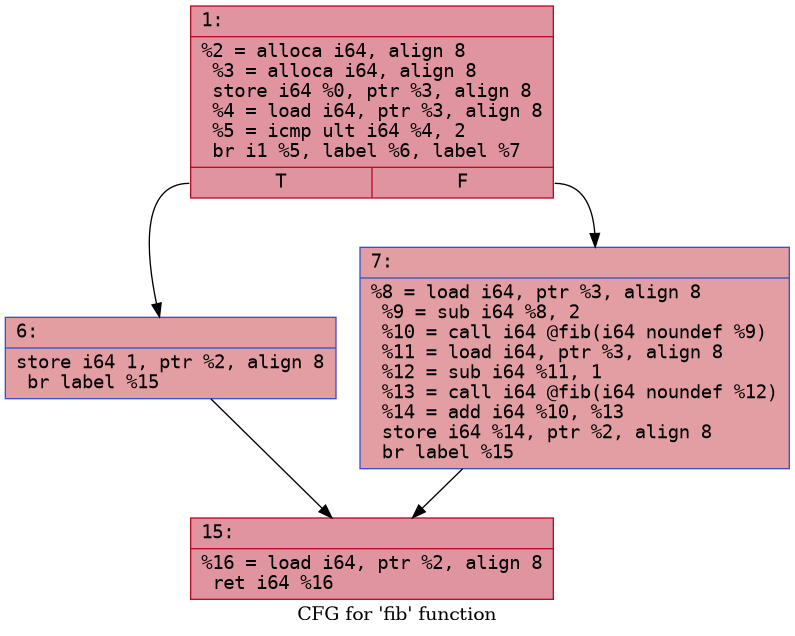
\includegraphics[width=0.5\linewidth]{fib2_.fib_O0.png}
    \caption{Grafo de fluxo de controle para a função '\textit{fib}' com nível 0 de otimização}
\end{figure}

\begin{figure}
    \centering
    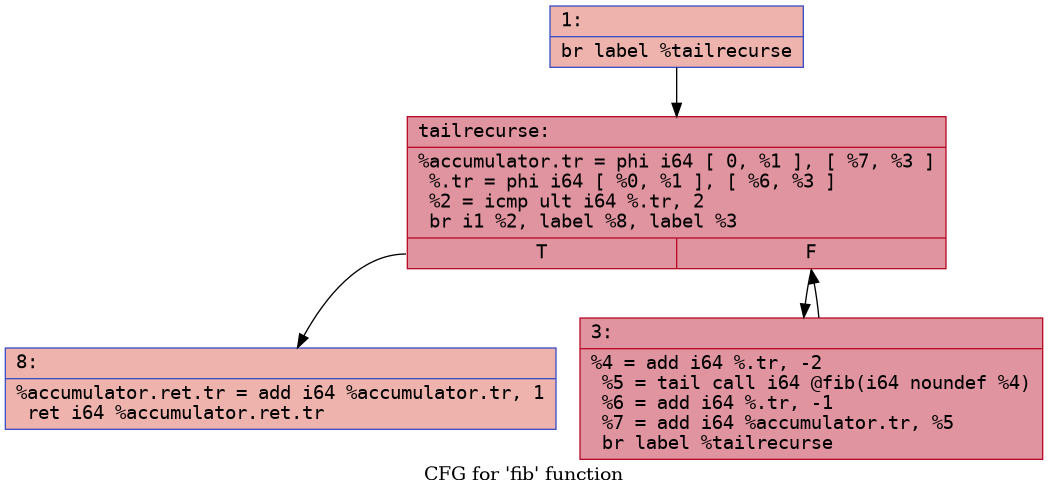
\includegraphics[width=0.5\linewidth]{fib2_.fib_O1.png}
    \caption{Grafo de fluxo de controle para a função '\textit{fib}' com nível 1 de otimização}
\end{figure}

\paragraph{}Em relação ao nível 2 de otimização, se comparado com o nível 1, é possível perceber que foi adicionado uma comparação inicial do valor passado à função ‘\textit{fib}’, por meio da instrução ‘\textit{icmp}’. Essa comparação garante que se na primeira vez que a função ‘\textit{fib}’ for chamada, caso seja passado um valor menor ou igual a 2, a função não irá executar instruções da recursão, aumentando a eficiência do programa.

\begin{figure}
    \centering
    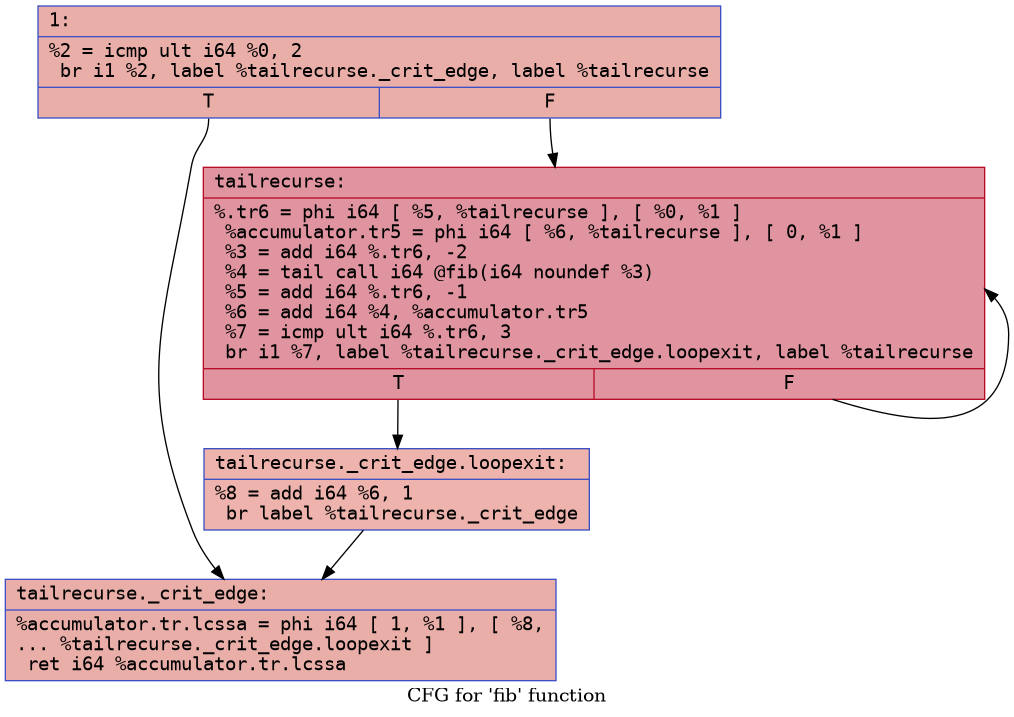
\includegraphics[width=0.5\linewidth]{fib2_.fib_O2.png}
    \caption{Grafo de fluxo de controle para a função '\textit{fib}' com nível 2 de otimização}
\end{figure}

\paragraph{}E em relação ao nível 3 de otimização, se comparado com o nível 2, não ocorreu nenhuma mudança no grafo de fluxo de controle.

\begin{figure}
    \centering
    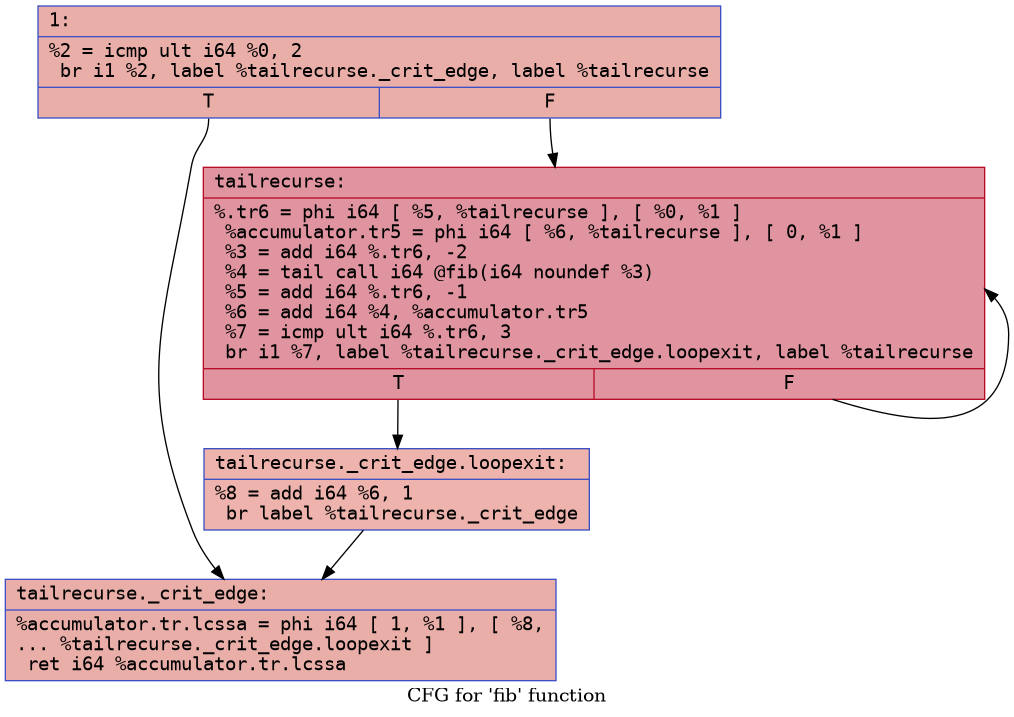
\includegraphics[width=0.5\linewidth]{fib2_.fib_O3.png}
    \caption{Grafo de fluxo de controle para a função '\textit{fib}' com nível 3 de otimização}
\end{figure}

\FloatBarrier

\subsection{\textit{Private}}

\paragraph{}Para a análise das técnicas de otimização de \textit{Private}, foi escolhida a função \textit{main}. Isso surge em virtude desta função apresentar um tipo específico de otimização pertinente ao programa \textit{Private}.

\begin{figure}
    \centering
    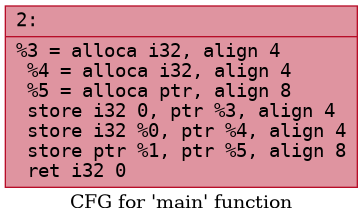
\includegraphics[width=0.5\linewidth]{private_.main_O0.png}
    \caption{Grafo de fluxo de controle para a função ‘\textit{main}’ com nível 0 de otimização.}
\end{figure}

\begin{figure}
    \centering
    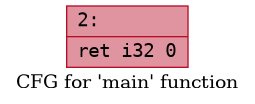
\includegraphics[width=0.5\linewidth]{private_.main_O1.png}
    \caption{Grafo de fluxo de controle para a função ‘\textit{main}’ com nível 1 de otimização.}
\end{figure}

\paragraph{}Como é possível perceber, no nível 1 de otimização, se comparado com a versão sem otimização, a função ‘\textit{main}’ deixou de executar as instruções de inicialização de uma função. Isso pode ser atribuído ao fato de que na ‘\textit{main}’, nada é executado, portanto essas instruções são desnecessárias.

\begin{figure}
    \centering
    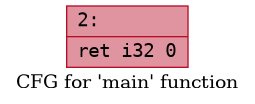
\includegraphics[width=0.5\linewidth]{private_.main_O2.png}
    \caption{Grafo de fluxo de controle para a função ‘\textit{main}’ com nível 2 de otimização.}
\end{figure}

\begin{figure}
    \centering
    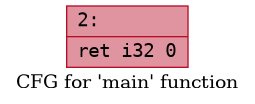
\includegraphics[width=0.5\linewidth]{private_.main_O3.png}
    \caption{Grafo de fluxo de controle para a função ‘\textit{main}’ com nível 3 de otimização.}
\end{figure}

\paragraph{}E em relação aos níveis 2 e 3 de otimização, não houve mudanças em relação ao nível 1.

\FloatBarrier

\subsection{\textit{Recursive}}

\paragraph{}Em relação ao programa \textit{Recursive}, para a análise das técnicas de otimização, foi escolhida a função ‘\textit{ack}’. A escolha dessa função deriva do fato dela ser uma das funções nas quais ocorrerão mais recursões.

\paragraph{}Uma das otimizações que pode ser percebida, no nível 1, é a redução do número de instruções do tipo ‘\textit{load}’ e ‘\textit{store}’, na \textit{label} filha à esquerda da primeira ramificação. Além disso, é possível notar que a \textit{label} filha à esquerda, na versão de nível 1 de otimização, está realizando diretamente o retorno da função, sem a necessidade de pular para a \textit{label} final. Isso é consequência de que na versão não otimizada, o valor do registrado da \textit{label} mais à esquerda da primeira ramificação, estava sendo armazenado na memória para depois ser carregado pela \textit{label} final, para realizar o retorno. Dessa forma essa otimização remove os \textit{loads} e \textit{stores} desnecessários, tornando o programa mais eficiente, por utilizar menos a memória e mais os registradores do processador.

\begin{figure}
    \centering
    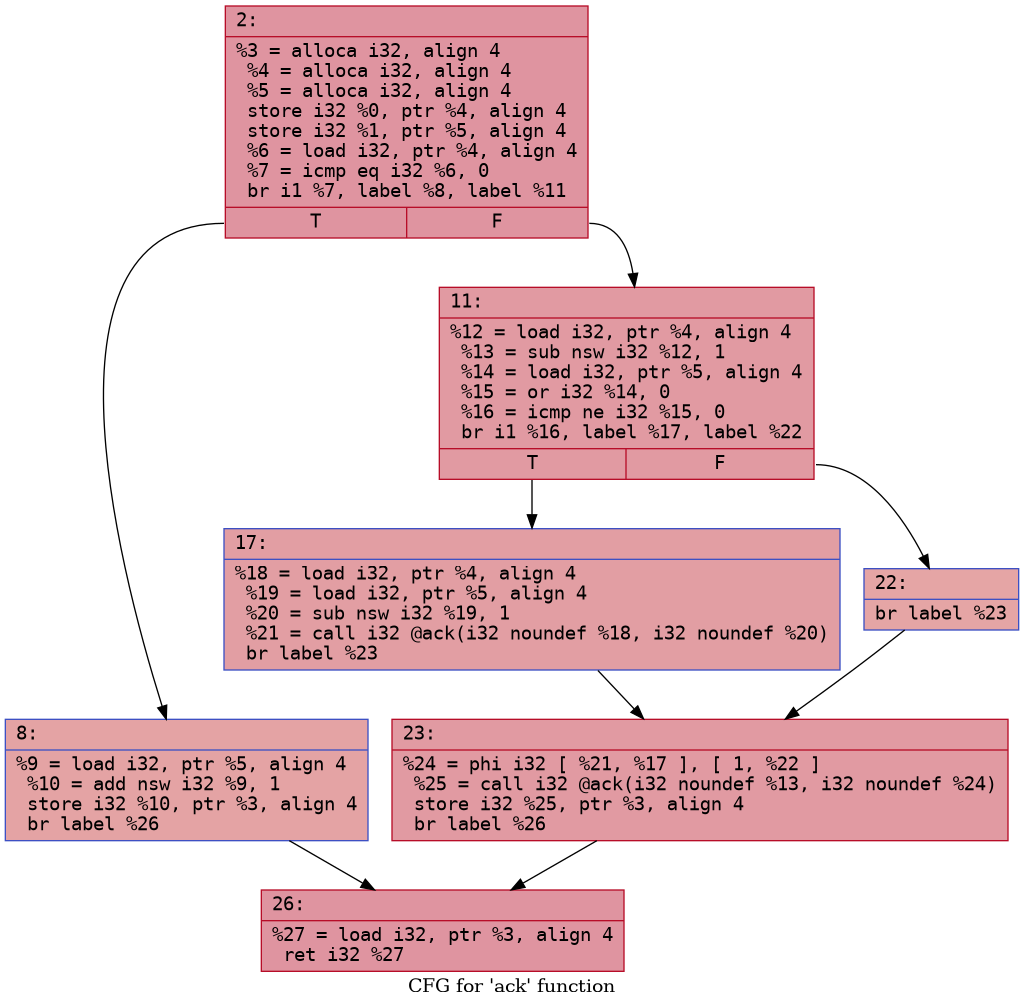
\includegraphics[width=0.5\linewidth]{recursive_.ack_O0.png}
    \caption{Grafo de fluxo de controle para a função ‘\textit{ack}’ com nível 0 de otimização.}
\end{figure}

\paragraph{}E em relação à otimização realizada no nível 2, em relação ao nível 1, é possível perceber, que de maneira semelhante a otimização de nível 2 da função ‘\textit{fib}’ do programa Fibonacci, visto anteriormente, foi adicionado uma comparação inicial do valor passado por parâmetro para a função ‘\textit{ack}’. Dessa forma, se o valor passado for igual a 0, o fluxo de execução do programa será direcionado para a \textit{label} final, dispensando a necessidade de atribuição estática de valor único, que não seria utilizada caso a função começasse com o valor de x igual à 0.

\begin{figure}
    \centering
    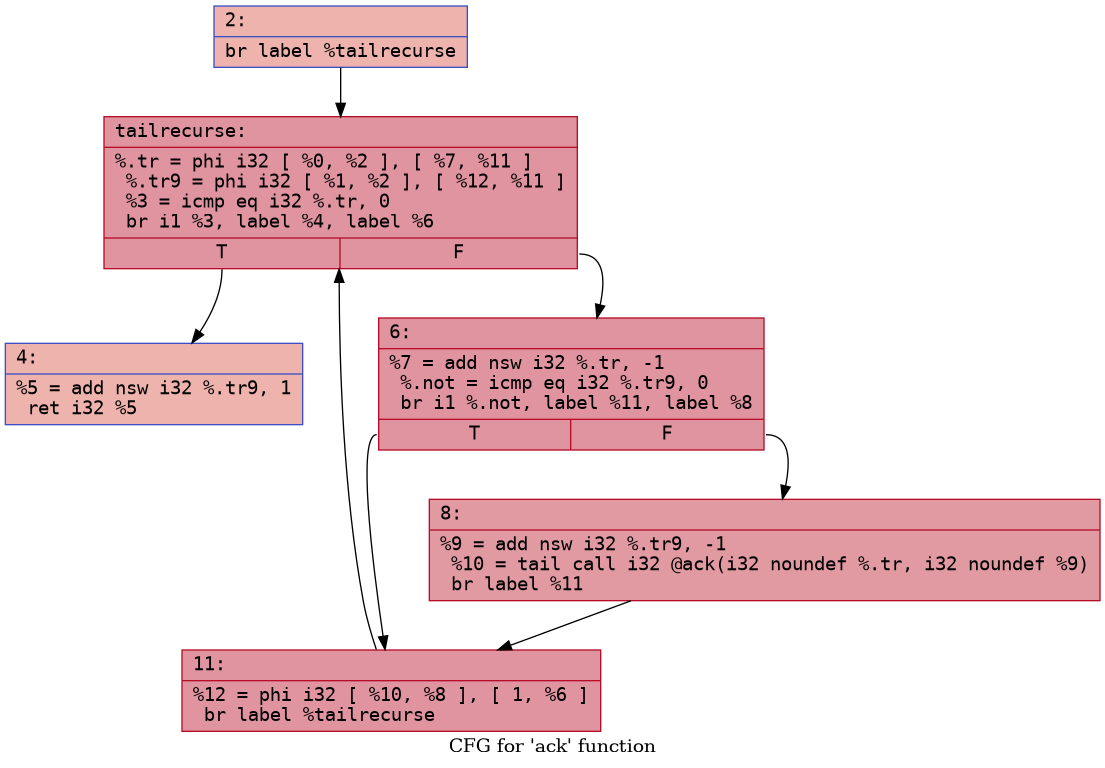
\includegraphics[width=0.5\linewidth]{recursive_.ack_O1.png}
    \caption{Grafo de fluxo de controle para a função ‘\textit{ack}’ com nível 1 de otimização.}
\end{figure}

\begin{figure}
    \centering
    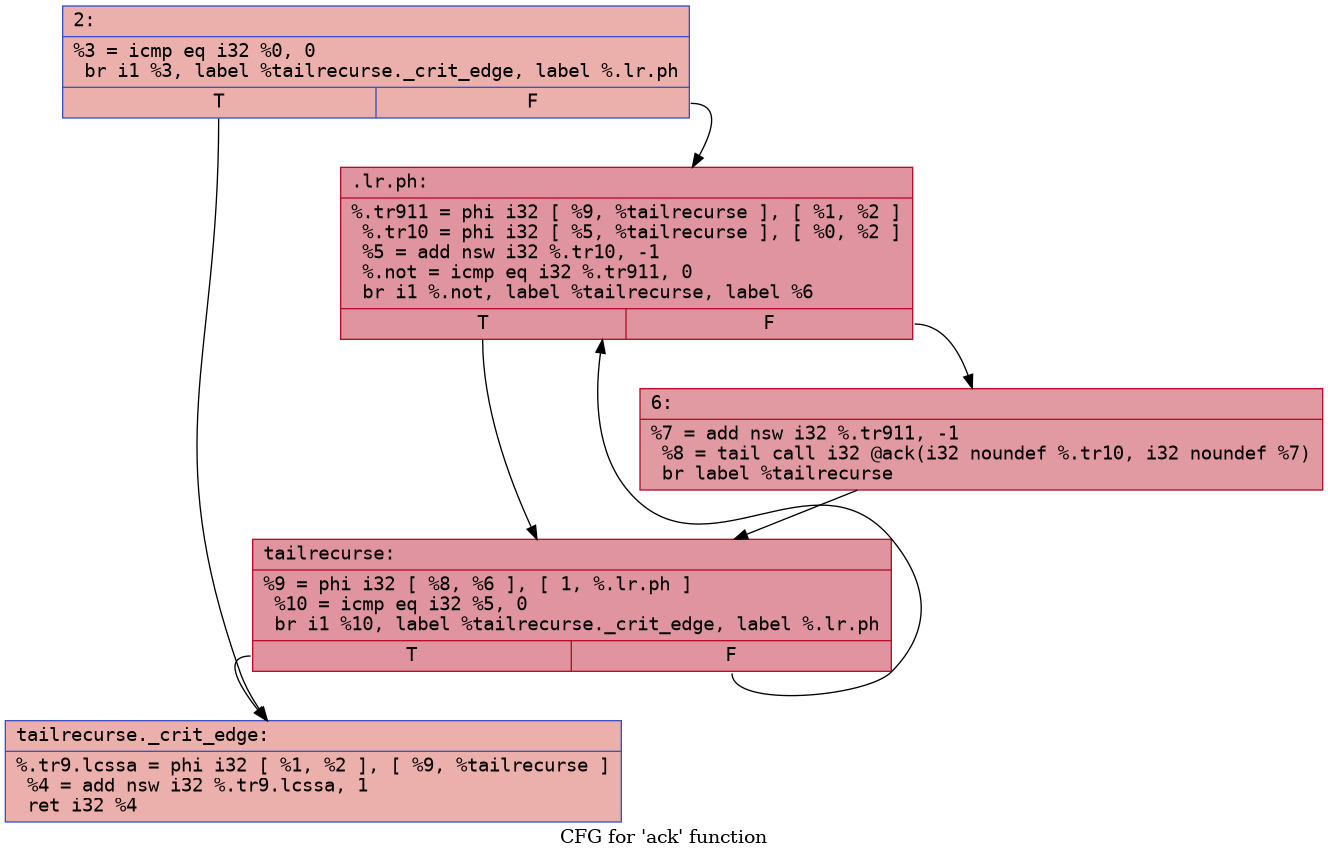
\includegraphics[width=0.5\linewidth]{recursive_.ack_O2.png}
    \caption{Grafo de fluxo de controle para a função ‘\textit{ack}’ com nível 2 de otimização.}
\end{figure}

\paragraph{}E em relação ao nível 3 de otimização, se comparado com o nível 2, não ocorreu nenhuma mudança no grafo de fluxo de controle.

\begin{figure}
    \centering
    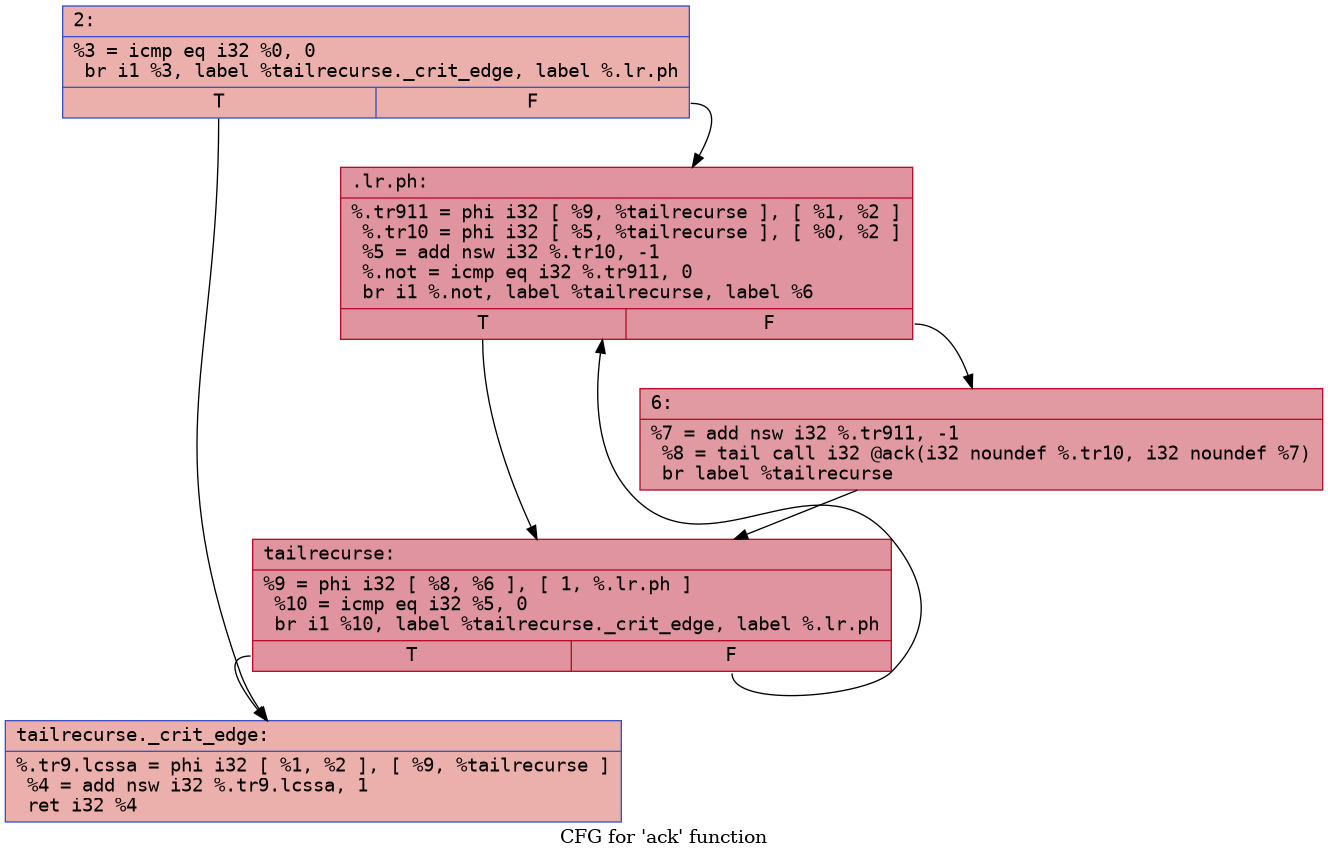
\includegraphics[width=0.5\linewidth]{recursive_.ack_O3.png}
    \caption{Grafo de fluxo de controle para a função ‘\textit{ack}’ com nível 3 de otimização.}
\end{figure}

\FloatBarrier

\section{Conclusão}

\paragraph{}Através deste trabalho foi possível compreender o funcionamento básico de um compilador de linguagens de programação, além dos diferentes níveis de otimização que o código intermediário sofre, permitindo, em última instância, a geração de um objeto executável otimizado para a máquina alvo.

\paragraph{}Além disso, foi possível compreender, em parte, o funcionamento de uma das ferramentas mais utilizadas na compilação de código fonte, que é o LLVM, e como é possível realizar o desenvolvimento de novos métodos de otimização para o código intermediário.

\end{document}
